\documentclass[rnd]{mas_proposal}
% \documentclass[thesis]{mas_proposal}

\usepackage[utf8]{inputenc}
\usepackage{amsmath}
\usepackage{amsfonts}
\usepackage{amssymb}
\usepackage{graphicx}

\title{Interactive Short Answer Grading}
\author{Mohandass Muthuraja, Jeeveeswaran Kishaan}
\supervisors{Prof. Paul G. Ploeger\\Deebul Nair }

% \thirdpartylogo{path/to/your/image}

\begin{document}

\maketitle

\pagestyle{plain}

\chapter{Introduction}
\begin{itemize}
    \item An introduction to the general topic you are covering.
    \item Why is it important? \\
\vspace*{1\baselineskip}

Interactive short answer grading deals with a human assisting the intelligent system for automatically grading the short answers. Short answers typically consist of one to few sentences. Automatic short answer grading drastically cuts down the effort of teachers. Many automated approaches have been proposed in the past for grading short answer questions. Though this approach was able to produce decent results, it suffers from the failure to capture the different wordings/phrasing of the students while trying to answer the short answer questions. These methods compare how similar the students' answers are and assign a grade proportional to the similarity of the students' answers to the answer provided by the professor. It is obvious that anticipating all different ways of answering his questions is practically impossible for the professor. Finding a way to understand the underlying concept of various students' answers and bagging the similar ones (or the right and wrong ones separately) is also a very tedious task. \\

This work proposes a method where a system tries to learn this task of measuring the correctness of each answer with the help of a human in the loop. During the learning stage, the system selects the predictions it’s least confident about and then asks the human expert for their correctness. Thus, it tries to reduce the human effort of going through all the answers while improving it's understanding of the problem on a iterative basis. \\

Active learning seems to be the best choice for this task as it actively queries the human for the grades of the samples it is most uncertain of.
Active learning is a new paradigm of learning where the learner queries the user/a human for the labels of certain data samples in such a way that it can learn to produce the desired outputs with higher accuracy. By actively selecting the data samples to label, it reduces a considerable amount of labeled training samples, thus, alleviating the problem of insufficient labeled data which is prevalent in supervised learning (where the correct labels for all kinds of inputs are available) approaches  
 

\end{itemize}





\section{Problem Statement}
\begin{itemize}
    \item What are you going to solve?
    \item How are you evaluating?
    
\vspace*{1\baselineskip}
    \item One of the biggest challenge involved in supervised learning in the need for large datasets. Generating a large data for short answer grading is also an obstacle. Many automatic short answer grading systems rely on supervised learning techniques. This, in turn, leads to high annotation cost of labeling the large training data. Also, the workload for labeling the data is more.
    \item As new data are generated on a regular basis, retraining the model for every new data also have a caveat of high computation cost.  Developing a generic model to overcome the deficit of retraining the model for every new answer can solve this issue.
    \item Short answer grading typically does not look for grammatical correctness and coherency. Short answers written by students have a lot of lexical diversity. Active learning can be used to handle the lexical diversity by involving human in training the model.
\end{itemize}


\chapter{Related Work}
\begin{itemize}
    \item What have other people done?
    \item Why is it not sufficient?
\end{itemize}

\section{Section 1}
\section{Section 2}



\chapter{Project Plan}

\section{Work Packages}
The bare minimum will include the following packages:
\begin{enumerate}
    \item[WP1] Literature Search
    \item[WP2] Experiments
    \item[WP3] Project Report
\end{enumerate}
Keep in mind that depending on your project, you will probably need to add work packages that are more suited to your projects.

\section{Milestones}
\begin{enumerate}
    \item[M1] Literature search
    \item[M2] Experimental setup
    \item[M3] Experimental Analysis
    \item[M4] Report submission
\end{enumerate}

\section{Project Schedule}
Include a gantt chart here. It doesn't have to be detailed, but it should include the milestones you mentioned above.
Make sure to include the writing of your report throughout the whole project, not just at the end.

\begin{figure}[h!]
    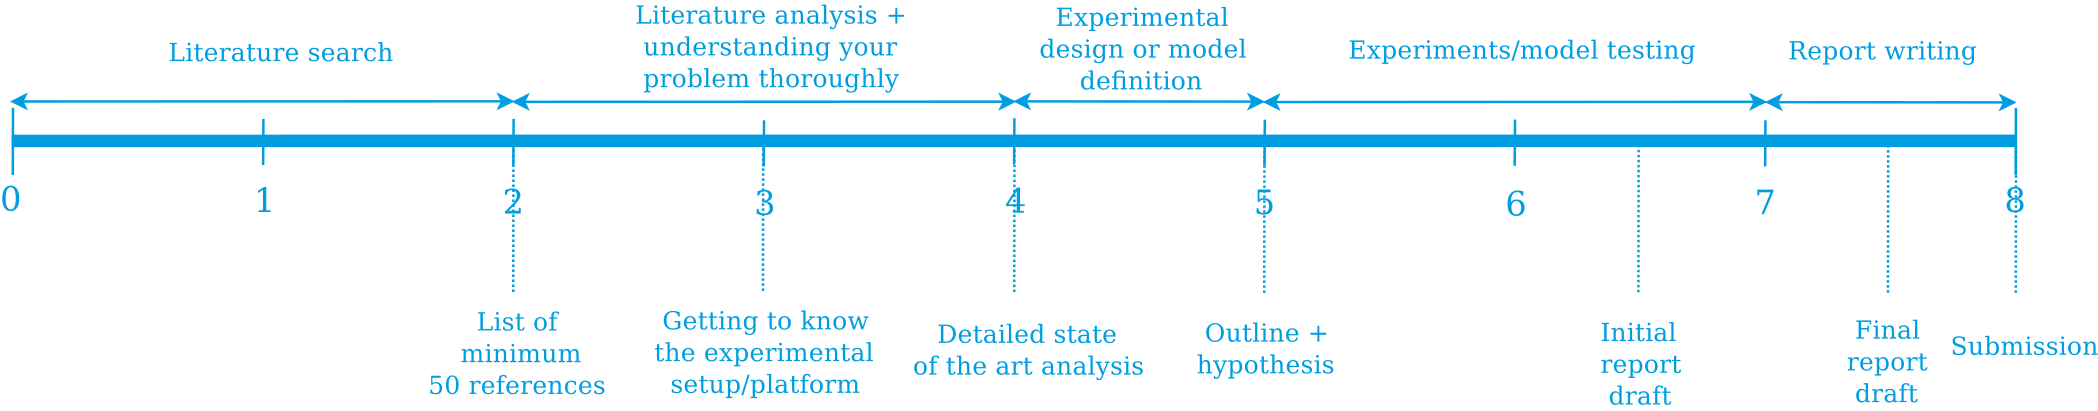
\includegraphics[width=\textwidth]{rnd_deliverable_timeline}
    \caption{}
    \label{}
\end{figure}

\section{Deliverables}
\subsection{Minimum Viable}

\begin{itemize}
    \item Survey the existing approaches for automatic short answer grading
    \item Review existing datasets for automatic short answer grading.
    \item Compile new datasets from different in-house domain
\end{itemize}

\subsection{Expected}
\begin{itemize}
    \item Evaluate the quality of different features for interactive short answer grading
    \item Evaluate Active Learning strategies for Short-Answer grading
    \item Implement a working model of 100 clicks for 1000 grades.
\end{itemize}

\subsection{Desired}
\begin{itemize}
    \item Integrate the best model with a graphical user interface(GUI)
\end{itemize}


\nocite{*}

\bibliographystyle{plainnat} % Use the plainnat bibliography style
\bibliography{bibliography.bib} % Use the bibliography.bib file as the source of references




\end{document}
